
In \cite{Landau:1935qbc}, Landau and Lifshitz proposed a description for the dynamics of the magnetisation vector\footnote{This is the direction in which the magnetic moment of a ferromagnet "prefers" to align.} in an isotropic ferromagnet. The eponymous \textit{Landau-Lifshitz} equation is given by 
\begin{equation}\tag{LL}\label{eq:LL}
	\partial_t u
		= -\alpha \big( u \times (u \times \Delta u)\big) + \beta \big( u \times \Delta u  \big),
\end{equation}
where $u : I \times \R^2 \to \SS^2$ is the \textit{magnetisation vector}. The parameter $\alpha \geq 0$ is the \textit{Gilbert damping}, representing the strength of dissipation in the model, while the parameter $\beta \in \R$ is the \textit{exchange constant}, representing the strength of dispersion. In the physics literature, the equation is often rescaled so that the parameters are balanced such that $\alpha^2 + \beta^2 = 1$, though mathematically this will be inconsequential for our discussion. 

From the perspective of geometric equations, the family of Landau-Lifshitz equations interpolates between the dispersive \textit{Schr\"odinger maps}, $(\alpha, \beta) = (1, 0)$, and the dissipative \textit{harmonic maps heat flow}, $(\alpha, \beta) = (0, 1)$, 
\begin{align}
	\partial_t u 
		&= \Delta u + |\nabla u|^2 u, 
		\tag{HMHF}\\
	\partial_t u 
		&= u\times \Delta u.
		\tag{SM}\label{eq:schrodinger}
\end{align}
The equation is naturally associated to the Dirichlet energy, 
	\[
		\cE[u] 
			:= \frac12 \int_{\R^2} |\partial_1 u|^2 + |\partial_2 u|^2 \, dx,
	\]
which, for
finite-energy (strong) solutions $u \in C^0_t \dot H^1_x (I \times \R^2)$ to the Landau-Lifshitz equation \eqref{LL}, satisfies the energy-balance identity 
	\begin{equation}\tag{E}\label{eq:energy}
	\cE[u(t)]
		+ 2 \alpha \int_0^t \int_{\R^2} |u \times (u \times \Delta u)|^2 \, dx ds = \cE[u_0].
	\end{equation}
In particular, the energy is non-increasing, and in fact conserved in the dispersive case. Both the equation \eqref{LL} and the Dirichlet energy are invariant under the rescaling 
\[ 
	u(t, x) \mapsto u(t/\lambda^2, x/\lambda),
\] 
i.e. \eqref{LL} is \textit{energy-critical}. It is then natural to study the dynamics of the Landau-Lifshitz equation \eqref{LL} in the energy topology $\dot H^1 (\R^2)$. The energy space further decomposes into infinitely-many connected components $\dot H^1_m (\R^2)$ indexed by their topological class $\deg(u) \equiv m$. The degree of a finite-energy map $u \in \dot H^1 (\R^2)$ is given by 
	\[
		\deg(u) := \frac{1}{4\pi}\int_{\R^2} u \cdot (\partial_1 u \times \partial_2 u) \, dx.
	\]
For continuous maps, the degree captures the number of times the plane wraps around the sphere under $u : \R^2 \to \SS^2$ (see Appendix \ref{appendix:bogo}).

The Landau-Lifshitz equation admits stationary solutions in the form of \textit{harmonic maps}. Remarkably, maps from the plane to the sphere $u : \R^2 \to \SS^2$ are \textit{self-dual} in the sense that the second-order harmonic maps equation admits a reduction to the first-order \textit{Cauchy-Riemann} equations. One can read off the reduction from the Bogomoln'yi identity (see Appendix \ref{appendix:bogo}),
\begin{equation}\tag{B}\label{eq:B}
	\cE[u]
		= \frac12 \int_{\R^2} |\partial_1 u - u \times \partial_2 u|^2 + 4\pi \deg(u).
\end{equation}
It follows that solutions to the Cauchy-Riemann equations 
	\begin{equation}\tag{HM}\label{eq:CR}
		\partial_1 u = u \times \partial_2 u,
	\end{equation}
are minimisers of Dirichlet energy within each topological class, i.e. the space of finite energy configurations with fixed degree $\deg(u) \equiv N$. The equations \eqref{CR} can be identified with usual formulation of the Cauchy-Riemann equations after stereographic projection $\SS^2 \to \C$, under which the solutions to \eqref{CR} correspond precisely to rational functions on $\C$. The basic $m$-equivariant solutions correspond to the maps $z \mapsto z^m$, taking the form 
\[
	Q^m (r, \theta) 
		:= e^{m \theta R} Q^m(r), 
		\qquad 
	Q^m (r) 
		:= 
			\begin{pmatrix} 
				h_1^m\\
				0\\
				h_3^m
			\end{pmatrix},
\]
where 
\begin{align*}
	h^m_1 (r) 
		:= \frac{2r^m}{r^{2m} + 1}, \qquad
	h^m_2 (r) 
		:= \frac{r^{2m} - 1}{r^{2m} + 1},
\end{align*}
and $R$ is the generator for rotation about the $z$-axis of the sphere $\SS^2$. 

In view of the energy-balance identity \eqref{energy}, variational heuristics suggest that harmonic maps are stable under the Landau-Lifshitz equation \eqref{LL} in the energy topology within each topological class. This is the main subject of this article. 

\subsection{Main result}

Following \cite{GustafsonEtAl2010}, we give an exposition on the \textit{asymptotic stability} of the \textit{harmonic maps} under the Landau-Lifshitz equation \eqref{LL} in \textit{equivariant symmetry}. 

To set the stage, the  $m$-equivariant maps take the form, 
	\[
		u (t, x) = e^{m \theta R} u(t, r),
	\]
where $R$ is the generator for rotation about the $z$-axis of the sphere $\SS^2$. For such maps, the energy norm reduces to 
	\[
		||u||_{\dot H^1_m}^2
			:= ||\partial_r u||_{L^2_x}^2 + || \tfrac{u}{r} ||_{L^2_x}^2. 
	\]

The Landau-Lifshitz equation \eqref{LL} is invariant under rotation, scaling, and translation. Observe that working in equivariant symmetry kills the last symmetry, so the \textit{moduli space of solitons} $\cQ_m \subseteq \dot H^1_m (\R^2)$ reduces to the two-dimensional family 
	\[
		\cQ_m
			:= \{ Q^m_{\alpha, \lambda} \in \dot H^1_{m} (\R^2): \alpha \in \SS^1 \text{ and } \lambda \in (0, \infty) \},
	\]
parametrised by the scaling parameter $\lambda \in (0, \infty)$ and rotation parameter $\alpha \in \SS^1$ as follows,
	\[
		Q^m_{\alpha, \lambda} (r, \theta) 
				:= e^{\alpha R} Q^m(r/\lambda, \theta). 
	\]

The problem of stability for $\cQ_m$ under \eqref{LL} concerns the dynamics of $m$-equivariant solutions to \eqref{LL} with energy close to the ground state, 
	\begin{equation}\label{eq:close}
		\cE[u] - \cE[Q^m] \ll 1. 
	\end{equation}
In \cite{gustafson2007schrodinger}, Gustafson-Kang-Tsai appled standard variational arguments to show that the family of harmonic maps $\cQ_m$ is \textit{orbitally stable} under the equation \eqref{LL} in the sense that solutions with energy close to the ground state, i.e. satisfying \eqref{close}, are in fact confined within a small neighborhood of the moduli space of solitons. More precisely,
	\begin{equation}\label{eq:orbital}
		\inf_{\alpha ,\lambda} || Q^m_{\alpha, \lambda} - u||_{\dot H^1}^2 \lesssim \cE[u] - \cE[Q^m] \ll 1. 
	\end{equation}


Projecting the solution onto $\cQ_m$, the solution schematically takes the form 
\begin{equation}\label{eq:decomp}
	u(t) = \underbrace{Q_{\alpha(t), \lambda(t)}}_{\text{projection to $\cQ_m$}} + \underbrace{\epsilon(t)}_{\text{small error in $\dot H^1$}}
\end{equation}
The orbital stability result \eqref{orbital} does not say much about the precise global dynamics of near solitons since scaling is a non-compact symmetry. Possibilities to consider include 
	\begin{itemize}
		\item Blow-up in either finite-time or infinite time, e.g. concentration into small scales,
			\[\lambda(t) \to 0,\]
		Finite-time blow-up is possible in the case $m = 1$, see \cite{merle2011blow,perelman2014blow}. Infinite-time blow-up is possible in the case $m = 2$, see \cite[Theorem 2]{GustafsonEtAl2010}.

		\item Breather-type solutions, e.g. oscillation between disparate scales, 
			\[
				\liminf \lambda(t) < \limsup \lambda(t). 
			\]
		This is possible in the case $m = 2$, see \cite[Theorem 2]{GustafsonEtAl2010}.

		\item Global existence and asymptotic stability, e.g. the modulation parameters converge and the error in \eqref{decomp} disperses, 
			\begin{align*}
				(\alpha(t), \lambda(t)) 
					\to (\alpha_\infty,\lambda_\infty),\qquad \text{and} \qquad
				||\epsilon||_{\cS_{t, x}([0, \infty) \times \R^2)} 
					< \infty.
			\end{align*}
		This holds for $m \geq 3$, see \cite[Theorem 1]{GustafsonEtAl2010}. 
	\end{itemize}
\begin{remark}
	Let us also point the interested reader to the results of Bejenaru-Tataru \cite{BejenaruTataru2014} on the case $m = 1$, and the recent preprint of Bejenaru-Tataru-Pillai \cite{bejenaru2024near} which deals with the most delicate case $m = 2$. 
\end{remark}

We are primarily interested in the asymptotic stabilty result of \cite[Theorem 1]{GustafsonEtAl2010} for Schr\"odinger maps \eqref{schrodinger}, i.e. the purely dispersive case of the Landau-Lifshitz equation \eqref{LL}. The dissipative case is an easy modification; 

\begin{figure}[h]
	\begin{center}
		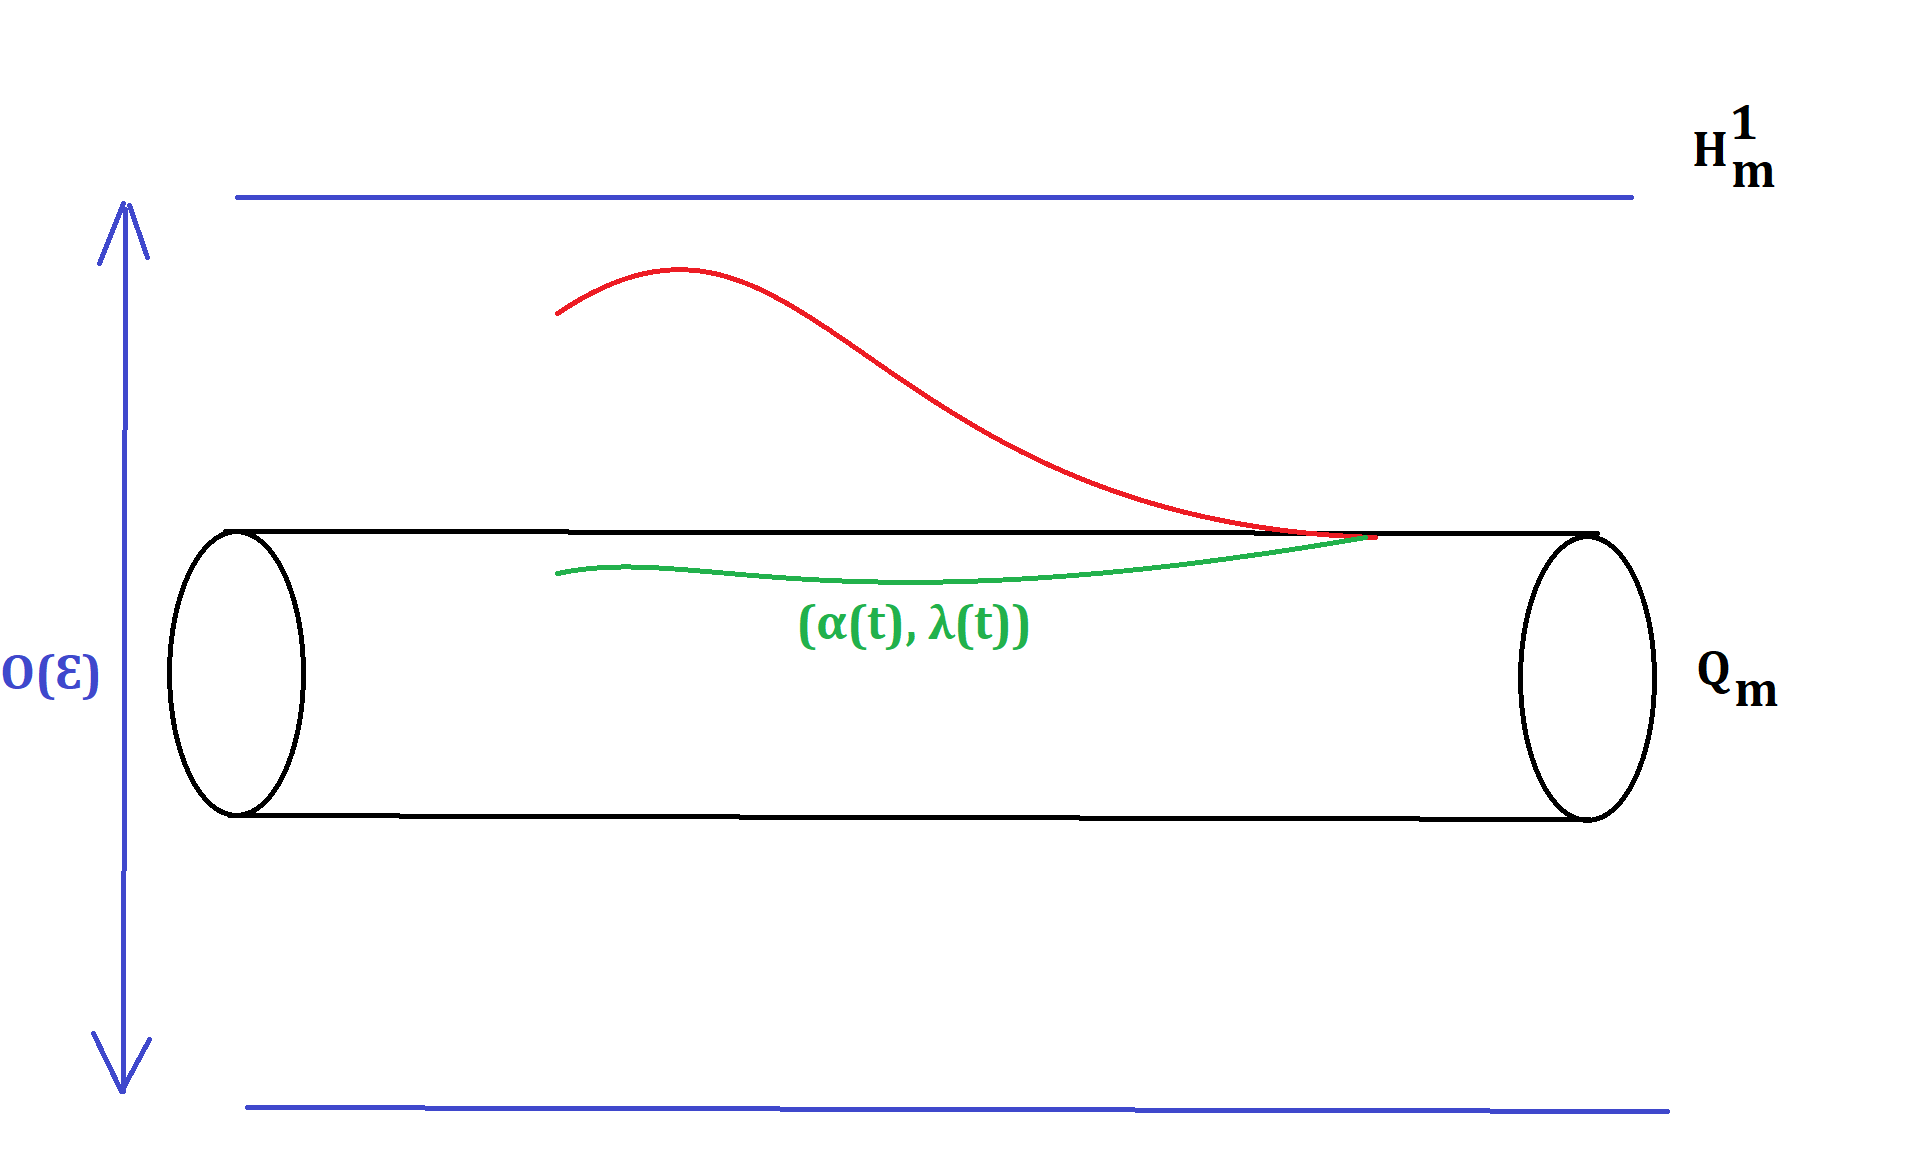
\includegraphics[scale=0.25]{graphics/moduli.png}
	\caption{The near soliton dynamics of \eqref{LL} can be decomposed into an ODE for the dynamics on the moduli space and a PDE for the error. }
\end{center}
\end{figure}

\begin{theorem}[Asymptotic stability of harmonic maps in equivariant symmetry]\label{thm:main}
	Let $m \geq 3$, then given initial data $u_0 \in \dot H^1_m (\R^2)$ with energy close to the ground state 
		\[
			\cE[u_0] - \cE[Q^m] \ll 1, 
		\]
	there exists a global solution $u \in C^0_t (\dot H^1_m)_x ([0, \infty) \times \R^2)$ to the Schr\"odinger maps equation \eqref{schrodinger} converging to a fixed soliton $Q^m_{\alpha_\infty, \lambda_\infty} \in \cQ_m$ in the sense that 
		\begin{equation}\label{eq:convergence}
			|| u (t) - Q_{\alpha_\infty, \lambda_\infty}||_{L^\infty_x} \overset{t \to \infty}{\longrightarrow} 0. 
		\end{equation}
\end{theorem}
